% =================================================================================================
% File:			archietettura.tex
% Description:	Defiinisce la sezione relativa a ...
% Created:		2015-02-23
% Author:		Tesser Paolo
% Email:		tesser.paolo@mashup-unipd.it
% =================================================================================================
% Modification History:
% Version		Modifier Date		Change											Author
% 0.0.1 		2015-02-23 			sistemato header								Tesser Paolo
% =================================================================================================
% 0.0.2			2015-03-26			modificata stesura e nuove aggiunte generiche	Tesser Paolo
% =================================================================================================
%

% CONTENUTO DEL CAPITOLO

\section{Descrizione Architettura} % (fold)
\label{sec:descrizione_architettura}

\subsection{Metodo e formalismo di specifica}
La descrizione dell'architettura dell'applicazione viene fornita con un approccio di tipo top-down: si descrive l'architettura partendo dal generale e si analizzano via via in dettaglio tutti i moduli che le compongono. Vengono forniti degli esempi d'utilizzo dei design pattern scelti. I diagrammi delle componenti, delle classi e i diagrammi di attività rispettano il formalismo di UML 2.0. \newline
Le classi i, framework usati dall'applicazione e le librerie utilizzate verranno marcate con colori diversi per facilitare la distinzione durante la consultazione. \newline
L’architettura generale non tratta l’intero insieme delle sottoclassi del sistema. Di conseguenza viene specificato lo scopo di una gerarchia e vengono individuate le relazioni con le varie componenti del sistema. Il resto dei dettagli viene rimandato alle diverse fasi di Progettazione di Dettaglio.


	\subsection{Architettura generale}
	L’architettura dell'applicazione segue il design pattern Three-Tier. Viene quindi suddivisa in tre livelli:
		\begin{enumerate}
			\item Client Tier;
			\item Server Tier;
			\item DataBase Tier.
		\end{enumerate}
		\noindent
		Di seguito viene proposto un diagramma rappresentante le relazioni tra i vari livelli. Vengono individuate le componenti che permettono ai vari livelli di interagire senza dover esporre la struttura interna degli stessi. \newline \newline

		[TO DO] (Diagramma con i tre livelli mostrati come package con all'interno annidati al package che si occupano della comunicazione tra i livelli) \newline \newline
		Come indicato nel diagramma, il livello del client interagisce con il server tramite gli EndPoints forniti dal Server. Esso riceverà e analizzerà la richiesta mediante [TO DO]. Una volta pronta, la risposta verrà fornita al Client.\newline
		Il client si occuperà di analizzarla per determinare se la richiesta ha avuto un esito positivo o negativo. Nel primo caso la gestione verrà delegata alla componente [TO DO]. \newline



		\subsubsection{Architettura Client Tier}
		Per il livello client è stato adottato il design pattern MVC offerto dal framework AngularJS. Questo livello implementa l'interfaccia grafica con cui utenti autenticati e amministratori possono interagire con il sistema in modo completo. Il diagramma seguente illustra l'interazione delle varie parti. \newline \newline

		[TO DO] (Diagramma che rappresenta il design pattern MVC) \newline \newline

		Gli utenti invocheranno determinate azioni utilizzando i pulsanti forniti dall'interfaccia e il sistema risponderà fornendo pagine di configurazione interattive oppure visualizzando una serie di grafici che verranno aggiornanti costantemente utilizzando i servizi REST forniti dall'applicazione tramite il modulo Processor [TO REVIEW]. In dettaglio:

		\begin{itemize}
			\item Model: TO DO;
			\item View: TO DO;
			\item Controller: TO DO.
		\end{itemize}

		\subsubsection{Architettura Server Tier}
		[TO REVIEW] Il livello server è composto da un modello e da una parte di comunicazione rappresentata dagli Endpoints forniti dalla piattaforma Google Cloud Engine. \newline \newline

		[TO DO] (Diagramma ancora da definire) \newline \newline
		[TO REVIEW] \newline
		La rappresentazione evidenzia il passaggio di dati e richieste che possono avvenire tra questo livello e gli altri presenti nell'applicazione.
		Una volta che il server riceve una richiesta REST, si occuperà di analizzarla ed elaborarla. Viene di conseguenza individuato l’oggetto o gli oggetti ai quali si riferisce e vengono estrapolati i dati effettivi della richiesta con una chiamata al livello Database. Questo individua la giusta operazione da eseguire, la quale analizzerà i dati associati alla richiesta ed li comunicherà al livello server. Viene infine fornita una risposta che verrà ritrasmessa all'oggetto che ha generato la richiesta REST.

		\subsubsection{Architettura Database Tier}
		Il livello database è gestito dal sistema Datastore integrato nella Google Cloud Platform che fornisce la funzionalità di persistenza dei dati. Ad esso spetta il compito di memorizzazione sia tutti i risultati recuperati dal Miner riguardanti i dati grezzi dei social, sia di memorizzare le configurazioni del programma necessarie al Processor e lo stato di lavoro dei Miner ad esso collegati.

		\subsubsection{Protocollo di comunicazione Client-Server}
		La comunicazione tra il livello Client e quello Server avviene tramite i Google Cloud Endpoints. Questi permettono di creare delle API da un'applicazione generata tramite la Google App Engine. Gli Endpoints garantiscono un modo semplice di sviluppare un back-end condiviso, riducendo di molto il lavoro che sarebbe necessario per implementare una simile infrastruttura. 
		\begin{comment}
		\begin{figure}[!htbp]
			\centering
			\centerline{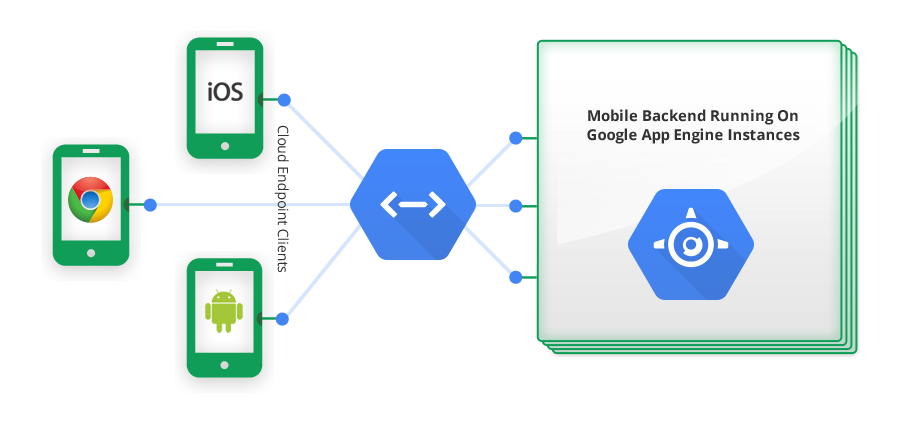
\includegraphics[scale=0.45]{./images/endpoints.png}}
			\caption{Modello generale di comunicazione Client-Server}
		\end{figure}
		\end{comment}

		\subsubsection{Protocollo di comunicazione Server-Database}
		La comunicazione tra il livello Server e quello del Database avviene tramite apposite funzionalità messe a disposizione dal servizio Datastore della piattaforma. Per poterle utilizzare il Server dovrà utilizzare il modulo: \textbf{google.appengine.ext.db}.


% section descrizione_architettura (end)